\documentclass{standalone}

%Til tikz billede
\usepackage{tikz}
\def\layersep{2.5cm}

\usetikzlibrary{shapes.multipart, matrix,chains,positioning,decorations.pathreplacing,shapes,arrows,arrows.meta}
\usetikzlibrary{arrows,decorations.pathmorphing,backgrounds,positioning,fit,petri}
% Til tyk skrift
\usepackage{bm}

% Til træer
% ggplot2 style tikz
\definecolor{obj}{gray}{0.95}
\definecolor{backG}{gray}{1}

\begin{document}

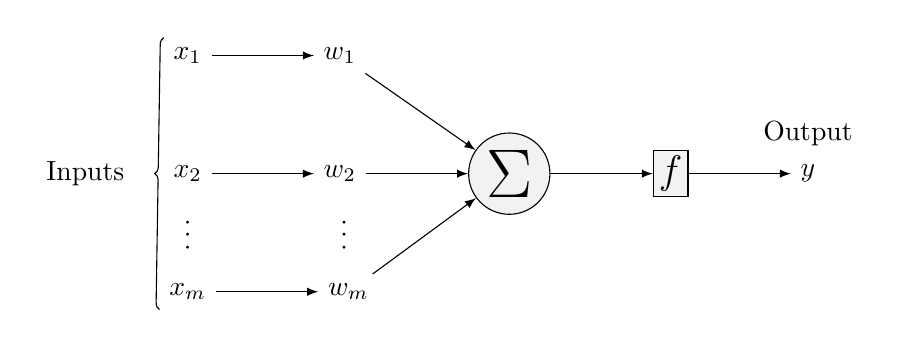
\begin{tikzpicture}[
	init/.style={
		draw,
		circle,
		inner sep=2pt,
		font=\Huge,
		join = by -latex
	},
	squa/.style={
		draw,
		inner sep=2pt,
		font=\Large,
		join = by -latex
	},
	start chain=2,node distance=13mm
	]
	\node[fill=backG,on chain=2] 
	(x2) {$x_2$};
	\node[fill=backG,on chain=2,join=by -latex] 
	(w2) {$w_2$};
	\node[fill=obj,on chain=2,init] (sigma) 
	{$\displaystyle\Sigma$};
	\node[fill=obj,on chain=2,squa,label=above:{\parbox{2cm}{}}]   
	{$f$};
	\node[fill=backG, on chain=2,label=above:Output,join=by -latex] 
	{$y$};
	\begin{scope}[start chain=1]
	\node[fill=backG, on chain=1] at (0,1.5cm) 
	(x1) {$x_1$};
	\node[fill=backG, on chain=1,join=by -latex] 
	(w1) {$w_1$};
	\end{scope}
	\begin{scope}[start chain=3]
	\node[fill=backG, on chain=3] at (0,-1.5cm) 
	(xm) {$x_m$};
	\node[fill=backG, on chain=3,join=by -latex] 
	(wm) {$w_m$};
	\end{scope}
	
	\path (x2) -- node[auto=false]{\rotatebox[origin=c]{90}{\ldots}} (xm);
	\path (w2) -- node[auto=false]{\rotatebox[origin=c]{90}{\ldots}} (wm);
	
	\draw[-latex] (w1) -- (sigma);
	\draw[-latex] (wm) -- (sigma);
	
	\draw[decorate,decoration={brace,mirror}] (x1.north west) -- node[fill=backG,left=10pt] {Inputs} (xm.south west);
	
	\begin{pgfonlayer}{background}
	\node [fill=backG,fit=(current bounding box.north west) (current bounding box.south east)] {};
	\draw[step=1cm,white,very thin] (current bounding box.north west) grid (current bounding box.south east);
	\end{pgfonlayer}
\end{tikzpicture}
\end{document}
